\section{Shende's argument}
In order to compare the Hodge structures of the De Rham and the Betti moduli spaces, we employ Shende's idea presented in \cite[]{Shende-weights}. The idea is to replace a complex manifold by a simplicial scheme and use this simplicial decomposition to give a presentation of the Betti moduli space as a simplicial scheme.
The main point of the construction is that, while the Betti moduli space doesn't admit a universal local system, since such a local system would not be of algebraic nature, this simplicial replacement does. As we saw in the previous system, universal bundles are the key to comparing the cohomology rings because the K\"unneth components of their Chern classes are generators.

In what follows, we will first explain in detail the idea behind Shende's construction. Then we will see how it applies to our case, when instead of a complex manifold as studied in \cite[]{Shende-weights} we have a stacky curve.

\subsection{A simplicial interpretation of the stack of local systems}
Let $X$ be a complex manifold, choose a base point $v_0 \in X$ for the fundamental group of $X$. For an algebraic group $G$, the stack of $G$-local systems on $X$ is the quotient
\begin{equation} \label{stack of local systems}
[\Hom(\pi_{1}(X, v_0), G) / G],
\end{equation}
where $\pi_{1}(X, v_0)$ is seen as a discrete algebraic group over $\Spec \mathbb{C}$.

Of course, the definition \eqref{stack of local systems} makes sense for any topological space $X$. By replacing $X$ with a simplicial decomposition, we can replace \eqref{stack of local systems} with an equivalent quotient stack.

Notice that we have a simplicial interpretation of the fundamental group. Indeed, if $\Delta_X$ is a simplicial set and $v_0 \in \Delta_X^0$ is a vertex, define $E(\Delta_X, v_0)$ the \textit{edge-path group} at $v_0$ as the group generated by loops of $1$-simplices pointed at $v_0$ under path-composition, modulo the relation killing boundaries of $2$-simplices
\begin{equation}
% Use \Biggl and \Biggr for larger angled parentheses 
% and \mid for a smaller separator than \middle|
E(\Delta_X, v_0) = \Biggl\langle
    \tikzpath{
      \node[dot, label=below:{\tiny $v_1$}] (v1) at (0.8,0) {};
      \node[dot, label=below:{\tiny $v_n$}] (vn) at (1.8,0) {};
      \node[dot, label=below:{\tiny $v_0$}] (v0e) at (2.6,0) {};
      \draw[-{Stealth}] (v0) -- (v1);
      \draw[dashed] (v1) -- (vn);
      \draw[-{Stealth}] (vn) -- (v0e);
    }
  \;\bigg|\;
  \begin{aligned}
      \tikzpath{
        \node[dot, label=below:{\tiny $v_n$}] (vn) at (1,0) {};
        \node[dot, label=below:{\tiny $v_0$}] (v0m) at (1.8,0) {};
        \node[dot, label=below:{\tiny $v'_1$}] (v1p) at (2.6,0) {};
        \node[dot, label=below:{\tiny $v'_{n'}$}] (vnp) at (3.8,0) {};
        \node[dot, label=below:{\tiny $v_0$}] (v0e) at (4.6,0) {};
        \draw[dashed] (v0) -- (vn);
        \draw[-{Stealth}] (vn) -- (v0m);
        \draw[-{Stealth}] (v0m) -- (v1p);
        \draw[dashed] (v1p) -- (vnp);
        \draw[-{Stealth}] (vnp) -- (v0e);
      }
    & = 
      \tikzpath{
        \node[dot, label=below:{\tiny $v'_{n'}$}] (vnp) at (1,0) {};
        \node[dot, label=below:{\tiny $v_0$}] (v0e) at (1.8,0) {};
        \draw[dashed] (v0) -- (vnp);
        \draw[-{Stealth}] (vnp) -- (v0e);
      }
      \cdot
      \tikzpath{
        \node[dot, label=below:{\tiny $v_n$}] (vn) at (1,0) {};
        \node[dot, label=below:{\tiny $v_0$}] (v0e) at (1.8,0) {};
        \draw[dashed] (v0) to (vn);
        \draw[-{Stealth}] (vn) -- (v0e);
      }
    , \\
    \begin{tikzpicture}[baseline={(v0.center)}, xscale=0.6, yscale=1]
      \tikzset{dot/.style={circle, fill, inner sep=0.8pt}}
      \node[dot] (v0) at (0,0) {}; 
      \node[dot] (v1) at (1,0) {}; \node[dot] (v2) at (2,0) {};
      \draw[-{Stealth}] (v0) -- node[below]{\tiny $\partial_2 \sigma$} (v1);
      \draw[-{Stealth}] (v1) -- node[below]{\tiny $\partial_0 \sigma$} (v2);
    \end{tikzpicture}
    & =
    \begin{tikzpicture}[baseline={(v0.center)}, xscale=0.6, yscale=1]
      \tikzset{dot/.style={circle, fill, inner sep=0.8pt}}
      \node[dot] (v0) at (0,0) {};
      \node[dot] (v1) at (1,0) {};
      \draw[-{Stealth}] (v0) -- node[below]{\tiny $\partial_1 \sigma$} (v1);
    \end{tikzpicture} \quad
    \forall \sigma \in X_2
  \end{aligned}
\Biggr\rangle.
\end{equation}

% \begin{equation}
% E(\Delta_X, v_0) = \left\langle
% % === 1. The Generator (Left Side) ===
%     \begin{tikzpicture}[baseline=-3pt]
%         \node[vdot] (1) {}; \node[lbl] at (1) {$v_0$};
%         \node[vdot] (2) [right=0.5cm of 1] {}; \node[lbl] at (2) {$v_1$};
%         \node (dots) [right=0.1cm of 2] {$\dots$};
%         \node[vdot] (3) [right=0.1cm of dots] {}; \node[lbl] at (3) {$v_n$};
%         \node[vdot] (4) [right=0.5cm of 3] {}; \node[lbl] at (4) {$v_0$};
        
%         \draw[arr] (1) -- (2);
%         \draw[arr] (3) -- (4);
%     \end{tikzpicture}
% \;\middle|\;
% \begin{aligned}
%     % === 2. The Long Relation (Concatenation) ===
%         \begin{tikzpicture}[baseline=-3pt]
%             % Chain: v0 -> ... -> vn -> v0 -> v'1 ... -> v'n' -> v0
%             \node[vdot] (a) {}; \node[lbl] at (a) {$v_0$};
%             \node (d1) [right=0.05cm of a] {$\dots$};
%             \node[vdot] (b) [right=0.05cm of d1] {}; \node[lbl] at (b) {$v_n$};
%             \node[vdot] (c) [right=0.5cm of b] {}; \node[lbl] at (c) {$v_0$};
%             \node[vdot] (d) [right=0.5cm of c] {}; \node[lbl] at (d) {$v'_1$};
%             \node (d2) [right=0.05cm of d] {$\dots$};
%             \node[vdot] (e) [right=0.05cm of d2] {}; \node[lbl] at (e) {$v'_{n'}$};
%             \node[vdot] (f) [right=0.5cm of e] {}; \node[lbl] at (f) {$v_0$};
            
%             \draw[arr] (a) -- (d1); \draw[arr] (d1) -- (b);
%             \draw[arr] (b) -- (c);
%             \draw[arr] (c) -- (d);
%             \draw[arr] (d) -- (d2); \draw[arr] (d2) -- (e);
%             \draw[arr] (e) -- (f);
%         \end{tikzpicture}
%     & = 
%         \begin{tikzpicture}[baseline=-3pt]
%             % Chain: v0 -> v'1 ... v'n' -> v0
%             \node[vdot] (a) {}; \node[lbl] at (a) {$v_0$};
%             \node[vdot] (b) [right=0.5cm of a] {}; \node[lbl] at (b) {$v'_1$};
%             \node (d) [right=0.05cm of b] {$\dots$};
%             \node[vdot] (c) [right=0.05cm of d] {}; \node[lbl] at (c) {$v'_{n'}$};
%             \node[vdot] (end) [right=0.5cm of c] {}; \node[lbl] at (end) {$v_0$};
            
%             \draw[arr] (a) -- (b);
%             \draw[arr] (b) -- (d); \draw[arr] (d) -- (c);
%             \draw[arr] (c) -- (end);
%         \end{tikzpicture}
%         \begin{tikzpicture}[baseline=-3pt]
%             % Chain: v0 ... vn -> v0
%             \node[vdot] (a) {}; \node[lbl] at (a) {$v_0$};
%             \node (d) [right=0.05cm of a] {$\dots$};
%             \node[vdot] (b) [right=0.05cm of d] {}; \node[lbl] at (b) {$v_n$};
%             \node[vdot] (c) [right=0.5cm of b] {}; \node[lbl] at (c) {$v_0$};
            
%             \draw[arr] (a) -- (d); \draw[arr] (d) -- (b);
%             \draw[arr] (b) -- (c);
%         \end{tikzpicture}
%       \\[1em]
%     % === 3. The Triangle and Boundary Equation ===
%     & \begin{tikzpicture}[baseline=0.2cm]
%             % Equation: dot -> dot -> dot = dot -> dot
%             % First arrow (d1)
%             \node[vdot] (a) {};
%             \node[vdot] (b) [right=0.8cm of a] {};
%             \draw[arr] (a) -- node[below, font=\scriptsize] {$\partial_1 \sigma$} (b);
            
%             % Second arrow (d0)
%             \node[vdot] (c) [right=0.8cm of b] {};
%             \draw[arr] (b) -- node[below, font=\scriptsize] {$\partial_0 \sigma$} (c);
            
%             % Equals
%             \node[right=0.2cm of c] (eq) {$=$};
            
%             % Third arrow (d2)
%             \node[vdot] (d) [right=0.2cm of eq] {};
%             \node[vdot] (e) [right=0.8cm of d] {};
%             \draw[arr] (d) -- node[below, font=\scriptsize] {$\partial_2 \sigma$} (e);
%       \end{tikzpicture}
% \end{aligned}
% \right\rangle
% \end{equation}

\begin{rmk} \label{iso fundamental group - edge-path group}
There is an isomorphism $\pi_1(|\Delta_X|, v_0) \simeq E(\Delta_X, v_0)$.
\end{rmk}

\begin{prop}\label{prop: stack of local systems - simplicial version}
Let X be a path-connected topological space. Suppose that $\pi_{1}(X, v_0)$ is finitely presented, e.g. if $X$ is a complex manifold. Let $\Delta_X$ be a simplicial set whose geometric realization is homotopy equivalent to $X$, having $v_0$ as a vertex. Call $X_i$ the $i$-th skeleton of $\Delta_X$.
Then the isomorphism $\pi_1(X, v_0) \simeq E(\Delta_X, v_0)$ induces an equivalence of quotient stacks
\begin{equation}
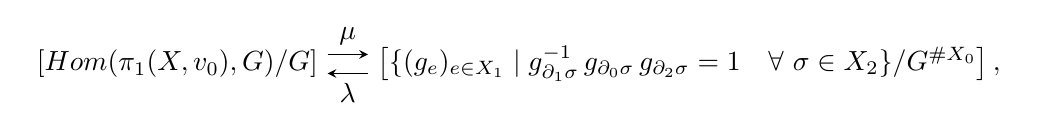
\begin{tikzpicture}[>=stealth]

  % Define the left node containing the Hom set quotient
  \node (left) at (0,0) {
    $\left[ \text{Hom}(\pi_1(X, v_0), G) / G \right]$
  };

  % Define the right node containing the set of functions
  \node (right) at (6.5,0) {
    $\left[ \{ (g_e)_{e \in X_1} \mid g_{\partial_1 \sigma}^{-1} 
            \, g_{\partial_0 \sigma} \, g_{\partial_2 \sigma} = 1 
            \quad \forall \ \sigma \in X_2 \} / G^{\# X_0} 
    \right],$
  };

  % Draw top arrow with mu label
  \draw[->, transform canvas={yshift=0.8ex}] (left) -- (right) 
    node[midway, above] {$\mu$};

  % Draw bottom arrow with lambda label below
  \draw[<-, transform canvas={yshift=-0.8ex}] (left) -- (right) 
    node[midway, below] {$\lambda$};

\end{tikzpicture}
\end{equation}
where $G^{\# X_0}$ acts on $F \coloneqq \left\{ (g_e)_{e \in X_1} \mid g_{\partial_1 \sigma}^{-1} \, g_{\partial_0 \sigma} \, g_{\partial_2 \sigma} = 1 \quad \forall \ \sigma \in X_2 \right\}$ by edge-boundaries, i.e.
\begin{equation}
(g_v)_{v \in X_0} \cdot (g_e)_{e \in X_1} = (g_{\partial_0 e} \, g_e \, g_{\partial_1 e}^{-1})_{e \in X_1}.
\end{equation}
\end{prop}

\begin{rmk}
Both $\Hom(\pi_1(X, v_0), G)$ and $F$ can be expressed as closed subvarieties of some $G^N$, so indeed the ones described in \zcref{prop: stack of local systems - simplicial version} are well defined algebraic stacks.
\end{rmk}

Using \zcref{iso fundamental group - edge-path group}, in proving \zcref{prop: stack of local systems - simplicial version} we replace $\pi_1(X, v_0)$ by $E \coloneqq E(\Delta_X, v_0)$.

\begin{proof}
We actually prove that the quotients prestacks are equivalent. Namely, we show that for $S$ scheme over $\mathbb{C}$ the groupoids
\begin{equation}
\begin{tikzcd}
	{G(S) \times \Hom(E, G)(S)} & {\Hom(E, G)(S)}
	\arrow[shift right, from=1-1, to=1-2]
	\arrow[shift left, from=1-1, to=1-2]
\end{tikzcd}
\end{equation}
and
\begin{equation}
\begin{tikzcd}
	{G(S)^{\# X_0} \times F(S)} & {F(S)}
	\arrow[shift right, from=1-1, to=1-2]
	\arrow[shift left, from=1-1, to=1-2]
\end{tikzcd}
\end{equation}
are equivalent, functorially in $S$.\\
On objects define $\lambda$ by
\begin{equation}
\begin{tikzpicture}
  % First row: The map definition
  \node (L1) at (0,0) [anchor=west] {
    $\lambda \colon F(S) \xrightarrow{\hspace{1.5cm}} \Hom(E, G)(S)$
  };
  % Second row: The element-wise mapping with labels shifted below bullets
  \node (L2) at (0,-0.8) [anchor=west] {
    $\underline{g}\coloneqq (g_e)_{e \in X_1} \mapsto \left[ 
      \varphi_{\underline{g}} \colon \graphfragment{} 
      \longmapsto g_{e_n} \cdot \dots \cdot g_{e_0} 
    \right].$
  };
\end{tikzpicture}
\end{equation}
Notice that $\varphi_{\underline{g}}$ is well defined because the conditions on the boundaries of $2$-simplices in $F$ and in $E$ are equivalent, and it is a group homomorphism by definition of the group operation in $E$, obtained by concatenating paths. Therefore $\lambda$ is well defined at the level of objects.
On morphisms, define $\lambda$ by
\begin{align}
\lambda \colon G(S)^{\# X_0} \times F(S) &\longrightarrow G(S) \times \Hom(E, G)(S) \\
  \left((g_v)_{v \in X_0}, (g_e)_{e \in X_1}\right) &\longmapsto (g_{v_0}, \varphi_{\underline{g}}).
\end{align}
Observe now that $\lambda$ is a morphism of groupoids, i.e. it commutes with source and target maps. The source map is the projection on the second factor in both groupoids, which commutes with $\lambda$ by definition. The target map is the group action, so compatibility with $\lambda$ means
\begin{equation} \label{eq: lambda action}
g_{v_0} \cdot \varphi_{\underline{g}} = \lambda\left((g_v)_v \cdot (g_e)_e \right).
\end{equation}
Since $(g_v)_v \cdot (g_e)_e = \left(g_{\partial_0 e} \, g_e \, g_{\partial_1 e}^{-1}\right)_e$, the right-hand side of \eqref{eq: lambda action} is the homomorphism
\begin{equation}
\begin{tikzpicture}[>=stealth, auto, node distance=1.2cm]
  % Row 1: Diagram maps to long product
  \node (start_graph) {\graphfragment{}};
  
  \node[right=0.2cm of start_graph] (mapsto) {$\longmapsto$};
  
  \node[right=0.2cm of mapsto] (product) {
    $( g_{v_0} \, g_{e_n} \, g_{v_n}^{-1} ) \,
     ( g_{v_n} \, g_{e_{n-1}} \, g_{v_{n-1}}^{-1} ) \, 
     \dots 
     ( g_{v_1} \, g_{e_0} \, g_{v_0}^{-1} )$
  };

  % Row 2: Simplified product
  \node[below=0.6cm of product.west, anchor=west] (simplified) {
    $= \quad g_{v_0} \, g_{e_n} \, g_{e_{n-1}} \dots g_{e_1} \, g_{e_0} \, g_{v_0}^{-1}$
  };

  % Row 3: Conjugation notation
  \node[below=0.8cm of simplified.west, anchor=west] (conjugation) {
    $= \quad g_{v_0} \cdot \varphi_{\underline{g}} \bigg( \graphfragment{} \bigg)$.
  };

\end{tikzpicture}
\end{equation}
This shows that $\lambda$ is a well defined morphism of groupoids.

Now define $\mu$. First, for any vertex $v \in X_1$ fix a path
\begin{equation}
\gamma_v \coloneqq 
\begin{tikzpicture}[baseline={(v.center)}, xscale=0.6, yscale=1]
    \tikzset{dot/.style={circle, fill, inner sep=0.8pt}}
    \node[dot, label=below:{\tiny $v$}] (v) at (0,0) {};
    \node[dot] (v1) at (1,0) {};
    \node[dot] (vn) at (2.2,0) {};
    \node[dot, label=below:{\tiny $v_0$}] (v0) at (3.2,0) {};
    \draw[-{Stealth}] (v) -- (v1);
    \draw[dashed] (v1) -- (vn);
    \draw[-{Stealth}] (vn) -- (v0);
\end{tikzpicture}.
\end{equation}
For simplicity assume $\gamma_{v_0}$ to be trivial. On objects, define $\mu$ by
\begin{align}
\mu\colon \Hom(E, G)(S) &\longrightarrow F(S) \\
(\varphi\colon E \to G(S)) &\mapsto \left(
\begin{tikzpicture}[baseline={(v.center)}, xscale=0.6, yscale=1]
    \tikzset{dot/.style={circle, fill, inner sep=0.8pt}}
    \node[dot, label=below:{\tiny $\partial_1 e$}] (v) at (0,0) {};
    \node[dot, label=below:{\tiny $\partial_0 e$}] (v') at (1,0) {};
    \draw[-{Stealth}] (v) -- node[above] {\tiny $e$} (v');
\end{tikzpicture}
\mapsto g_e^{\varphi} \coloneqq \varphi (\gamma_{\partial_0 e} * e * \gamma_{\partial_1 e}^{-1})
\right).
\end{align}
Notice that $(g_e^{\varphi})_{e \in X_1}$ as defined above does belong to $F(S)$ because of the relations on boundaries of $2$-simplices in $E$. On morphisms, define $\mu$ by
\begin{align}
\mu \colon G(S) \times \Hom(E, G)(S) &\longrightarrow G(S)^{\# X_0} \times F(S) \\
(g, \varphi) & \mapsto \left((g)_{v \in X_0}, (g_e^{\varphi})_{e \in X_1}\right).
\end{align}
As before, the compatibility of $\mu$ with the source maps is trivial, so we only need to check commutativity with the group actions, which holds by the following computation
\begin{multline}
\mu(g \cdot \varphi) = \mu(g \, \varphi \, g^{-1}) = (g_e^{g \varphi g^{-1}})_{e \in X_1} = (g \, (\gamma_{\partial_0 e} * e * \gamma_{\partial_1 e}^{-1}) \, g ^{-1})_{e \in X_1} \\
= (g \, g_e^{\varphi} \, g^{-1})_{e \in X_1} = (g)_{v \in X_0} \cdot (g_e^{\varphi})_{e \in X_1}.
\end{multline}

Finally, we need to show that $\lambda$ and $\mu$ are inverse equivalences. We show that the two compositions are naturally isomorphic to the identity. Since the only nontrivial part of the definition of both $\lambda$ and $\mu$ comes from the definition on objects, it suffices to show that the two compositions give the identity on objects. The first composition is
\begin{equation}
\lambda \circ \mu (\varphi)
= \lambda((g_e^{\varphi})_{e \in X_1})
% = \lambda( (\varphi(\gamma_{v_0}*e*\gamma_{v_1}))_{e \in X_1} )
= \left[
\graphfragment{}
\mapsto g_{e_n}^{\varphi} \dots g_{e_0}^{\varphi}\right].
\end{equation}
The triviality follows from
\begin{align}
g_{e_n}^{\varphi} \cdot \dots \cdot g_{e_0}^{\varphi} &= \varphi(\gamma_{v_0}*e_n*\gamma_{v_n}^{-1}) \, \varphi(\gamma_{v_n}*e_{n-1}*\gamma_{v_{n-1}}^{-1}) \dots \varphi(\gamma_{v_1}*e_0*\gamma_{v_0}^{-1}) \\
& = \varphi(\gamma_{v_0}*e_n*\gamma_{v_n}^{-1} * \gamma_{v_n}*e_{n-1}*\gamma_{v_{n-1}}^{-1} * \dots * \gamma_{v_1}^{-1} \gamma_{v_1}*e_0*\gamma_{v_0}^{-1}) \label{trivial comp step 1}\\
& = \varphi ( e_n * e_{n-1} * \dots * e_0 ), \label{trivial comp step 2}
\end{align}
where the first equality is because $\varphi$ is a group homomorphism and the second is because $\gamma_{v_0}$ is trivial.\\
Finally, we compute the other composition
\begin{equation}
\mu \circ \lambda (\underline{g}) = \mu(\varphi_{\underline{g}}) = \big(g_e^{\varphi_{\underline{g}}}\big)_{e \in X_1} = \big(\varphi_{\underline{g}}(\gamma_{\partial_0 e} * e * \gamma_{\partial_1 e}^{-1})\big)_{e \in X_1}.
\end{equation}
For $\gamma_v =
\begin{tikzpicture}[baseline={(v.center)}, xscale=0.6, yscale=1]
    \tikzset{dot/.style={circle, fill, inner sep=0.8pt}}
    \node[dot, label=below:{\tiny $v$}] (v) at (0,0) {};
    \node[dot, label=below:{\tiny $v_1$}] (v1) at (1,0) {};
    \node[dot, label=below:{\tiny $v_m$}] (vn) at (2.2,0) {};
    \node[dot, label=below:{\tiny $v_0$}] (v0) at (3.2,0) {};
    \draw[-{Stealth}] (v) -- node[above] {\tiny $a_0$} (v1);
    \draw[dashed] (v1) -- (vn);
    \draw[-{Stealth}] (vn) -- node[above] {\tiny $a_m$} (v0);
\end{tikzpicture}$, define $g_{\gamma_v} \coloneqq g_{a_m}\dots g_{a_0}$. Then
\begin{equation}
\varphi_{\underline{g}}(\gamma_{\partial_0 e} * e * \gamma_{\partial_1 e}^{-1}) = g_{\gamma_{\partial_0 e}} \, g_e \, g_{\gamma_{\partial_1 e}^{-1}}.
\end{equation}
Therefore
\begin{equation}
\mu \circ \lambda (\underline{g}) = \left(g_{\gamma_{\partial_0 e}} \, g_e \, g_{\gamma_{\partial_1 e}^{-1}}\right)_{e \in X_1} = (g_{\gamma_v})_{v \in X_0} \cdot (g_e)_{e \in X_1}.
\end{equation}
So the action by $ (g_{\gamma_v})_{v \in X_0} \in G(S)^{\# X_0} $ defines a natural isomorphism $\mu \circ \lambda \xRightarrow{\sim} \text{id}$.

Notice that throughout the argument we never made any choices of elements in $G(S)$. Indeed, the only choice were the paths $\gamma_v$. For this reason, the constructed equivalences are functorial in $S$ and hence lift to an isomorphism of the quotient prestacks, lifting to an isomorphism of the quotient stacks.
\end{proof}

Now we want to define a third equivalent stack to the stack of local systems. Actually, \zcref{prop: stack of local systems - simplicial version} is just an intermediate step and not the equivalence used in \cite{Shende-weights}.\\
Recall that any algebraic stack can be thought of as a smooth groupoid in algebraic spaces, and in particular it can be extended to a simplicial algebraic space by taking iterated fibered products of an atlas over the base. For example, the classifying stack $BG$ can be realized as
\begin{equation}
\begin{tikzcd}
	\dots & {G \times G} && G & {\Spec k.}
	\arrow["\vdots"'{yshift=5pt}, shift left, from=1-1, to=1-2]
	\arrow["{d_1 = m}"{description}, from=1-2, to=1-4]
	\arrow["{d_0 = pr_1}", shift left=3, from=1-2, to=1-4]
	\arrow["{d_2 = pr_2}"', shift right=3, from=1-2, to=1-4]
	\arrow[shift right=2, from=1-4, to=1-5]
	\arrow[shift left=2, from=1-4, to=1-5]
\end{tikzcd}
\end{equation}

\begin{rmk}\cite[See][Lemma 3.5]{SimplicialHomotopyTheory} \label{BG is 2-coskeleton}
The simplicial classifying space $BG$ has the property that for any simplicial scheme $Y$, a simplicial map $Y \to BG$ is determined by its components of degree up to two. More explicitly, the set of simplicial maps $ f \colon Y \to BG$ is in bijection with the set of truncated diagrams
\begin{equation} \label{eq: maps to BG}
\begin{tikzcd}
	{Y_2} & {Y_1} & {Y_0} \\
	{G \times G} & G & {\Spec k,}
	\arrow[from=1-1, to=1-2]
	\arrow[shift left=3, from=1-1, to=1-2]
	\arrow[shift right=3, from=1-1, to=1-2]
	\arrow["{f_2}", from=1-1, to=2-1]
	\arrow[shift right=2, from=1-2, to=1-3]
	\arrow[shift left=2, from=1-2, to=1-3]
	\arrow["{f_1}", from=1-2, to=2-2]
	\arrow[from=1-3, to=2-3]
	\arrow[from=2-1, to=2-2]
	\arrow[shift left=3, from=2-1, to=2-2]
	\arrow[shift right=3, from=2-1, to=2-2]
	\arrow[shift right=2, from=2-2, to=2-3]
	\arrow[shift left=2, from=2-2, to=2-3]
\end{tikzcd}
\end{equation}
where $f_1$ and $f_2$ commute with face and degeneracy maps. Note moreover that, since the projections $G \times G \to G$ are face maps, the value of $f_2$ is uniquely determined by the value of $f_1$, but the existence of $f_2$ imposes conditions on $f_1$ due to the compatibility with the multiplication in $G$. It follows that the set of simplicial maps $f \colon  Y \to BG$ is in bijection with the set of morphisms $f_1 \colon  Y_1 \to G$ which can be extended (necessarily uniquely) to \eqref{eq: maps to BG}.
\end{rmk}


The simplicial set $\Delta_X$ can also be given the structure of a simplicial scheme, by replacing every simplex by $\Spec k$
% The case we are interested in is when $X$ is a complex curve. In this case, there are no simplices of dimension greater than two and therefore $\Delta_X$ is degenerate in degree greater than two and can be realized as a simplicial scheme as
\begin{equation}
\begin{tikzcd}
	{\Delta_{X}} & \dots & {\coprod_{X_2} \Spec k} & {\coprod_{X_1} \Spec k} & {\coprod_{X_0} \Spec k.}
	\arrow["{=}"{marking, allow upside down}, draw=none, from=1-1, to=1-2]
	\arrow["\vdots"'{yshift=5pt}, shift left, from=1-2, to=1-3]
	\arrow[from=1-3, to=1-4]
	\arrow[shift left=3, from=1-3, to=1-4]
	\arrow[shift right=3, from=1-3, to=1-4]
	\arrow[shift right=2, from=1-4, to=1-5]
	\arrow[shift left=2, from=1-4, to=1-5]
\end{tikzcd}
\end{equation}

Consider now the presheaf of groupoids $\shHom_{SSch}(\Delta_X, BG)^{\text{pre}}$. Explicitly, the objects over $S$ are
\begin{equation}
\shHom_{SSch}(\Delta_X, BG)^{\text{pre}}(S) \coloneqq \Hom_{SSch}(\Delta_{X, S}, BG),
\end{equation}
where $\Delta_{X,S}$ is the fibered product over $\Spec k$ of $\Delta_X$ with $S$, i.e.
\begin{equation}
\begin{tikzcd}
	{\Delta_{X,S}} & \dots & {\coprod_{X_2} S} & {\coprod_{X_1} S} & {\coprod_{X_0} S.}
	\arrow["{=}"{marking, allow upside down}, draw=none, from=1-1, to=1-2]
	\arrow["\vdots"'{yshift=5pt}, shift left, from=1-2, to=1-3]
	\arrow[from=1-3, to=1-4]
	\arrow[shift left=3, from=1-3, to=1-4]
	\arrow[shift right=3, from=1-3, to=1-4]
	\arrow[shift right=2, from=1-4, to=1-5]
	\arrow[shift left=2, from=1-4, to=1-5]
\end{tikzcd}
\end{equation}
This is made into a groupoid by considering homotopies of simplicial morphisms. Namely, if $f,f' \in \Hom_{SSch}(\Delta_{X, S}, BG)$, an isomorphism $f \xrightarrow{\sim} f'$ will be a homotopy such that $d_0^{n+1} h_0^n = f_n$ and $d_{n+1}^{n+1} h_n^n = f'_n$ for all $n$.

Notice that, since $BG$ is a Kan complex, homotopy of maps into $BG$ is indeed an equivalence relation \cite[Corollary 6.2]{SimplicialHomotopyTheory}, therefore $\Hom_{SSch}(\Delta_{X, S}, BG)$ is a well defined groupoid. Then we can define $\shHom_{SSch}(\Delta_X, BG)$ as the stackification of $\shHom_{SSch}(\Delta_X, BG)^{\text{pre}}$.

\begin{thm} \label{thm: stack of local systems as stack of simplicial maps}
There is an isomorphism of stacks
\begin{equation}
\left[ \text{Hom}(\pi_1(X, v_0), G) / G \right] \cong \shHom_{SSch}(\Delta_X, BG)
\end{equation}
between the stack of local systems on $X$ and the stack of simplicial morphisms of $\Delta_X$ into the classifying stack $BG$.
\end{thm}
\begin{proof}
Using \zcref{prop: stack of local systems - simplicial version}, it suffices to show the existence of an isomorphism
\begin{equation}
\left[ F / G^{\# X_0} \right] \cong \shHom_{SSch}(\Delta_X, BG).
\end{equation}
As before, we actually show the existence of an isomorphism of the prestacks
\begin{equation}
\left[ F / G^{\# X_0} \right]^{\text{pre}} \cong \shHom_{SSch}(\Delta_X, BG)^{\text{pre}},
\end{equation}
i.e. an isomorphism of groupoids
\begin{equation}
\left[ F / G^{\# X_0} \right]^{\text{pre}}(S) \cong \Hom_{SSch}(\Delta_{X, S}, BG),
\end{equation}
functorial in $S$. Consider $f \in \Hom_{SSch}(\Delta_{X, S}, BG)$. By \zcref{BG is 2-coskeleton} this is equivalent the datum of
\begin{equation}
f_2 \colon \coprod_{X_2} S \to G \times G \quad \text{and} \quad f_1 \colon \coprod_{X_1} S \to G,
\end{equation}
respecting face and degeneracy maps. These correspond to choices of elements $(l_{\sigma}, l'_{\sigma})_{\sigma \in X_2} \in (G(S) \times G(S))^{\# X_2}$ and $(g_e)_{e \in X_1} \in G(S)^{\# X_1}$. The compatibility with face maps gives the conditions
\begin{equation}
g_{\partial_0 \sigma} = l_{\sigma}, \quad g_{\partial_1 \sigma} = l_{\sigma} \, l'_{\sigma}, \quad g_{\partial_2 \sigma} = l'_{\sigma}.
\end{equation}
Therefore, the morphism $f$ is uniquely determined by the choice of $(g_e)_{e \in X_1}$ such that $g_{\partial_1 \sigma}^{-1} \, g_{\partial_0 \sigma} \, g_{\partial_2 \sigma}  = 1$ for all $2$-simplices $\sigma$. Therefore the groupoids $\Hom_{SSch}(\Delta_{X, S}, BG)$ and $\left[ F / G^{\# X_0} \right]^{\text{pre}}(S)$ have the same objects. We now want to show that they also have the same groupoid structure, i.e. that homotopies on the left-hand side correspond to the action of $G(S)^{\# X_0}$ on $F(S)$.
Consider therefore two morphisms $f, f' \in \Hom_{SSch}(\Delta_{X,S}, BG)$. A homotopy $H \colon f \Rightarrow f'$ is a simplicial map $H \colon \Delta_{X,S} \times \Delta^1 \to BG$ such that
\begin{equation}
\begin{tikzcd}
	{\Delta_{X,S} \cong \Delta_{X,S} \times \Delta^0} \\
	{\Delta_{X,S} \times \Delta^1} && BG \\
	{\Delta_{X,S} \cong \Delta_{X,S} \times \Delta^0}
	\arrow["{id \times s_1}"', from=1-1, to=2-1]
	\arrow["f", from=1-1, to=2-3]
	\arrow["H"{pos=0.4}, from=2-1, to=2-3]
	\arrow["{id \times s_0}", from=3-1, to=2-1]
	\arrow["{f'}"', from=3-1, to=2-3]
\end{tikzcd}
\end{equation}
commutes. Giving $H$ is equivalent to giving for all $n$ a family of morphisms $h^n_i \colon (\Delta_{X,S})_n \to (BG)_n$ for $i = 0, \dots, n$ satisfying suitable compatibility conditions with face and degeneracy maps. Explicitly, the relationship between $H$ and $h$ is given by
\begin{equation} \label{eq: homotopy}
h^n_j = H^{n+1}_{j+1} \, s^n_j \quad \text{for } j=0,\dots, n.
\end{equation}
\zcref{BG is 2-coskeleton} shows that $H$ is determined by its degree one part, with degree two giving a compatibility condition. Then \zcref{eq: homotopy} shows that the morphisms $h^n_j$ are determined by the degree zero part, with degree one giving a compatibility condition.\\
Let $f, f' \in \Hom_{SSch}(\Delta_{X, S}, BG)$ be simplicial maps and let $h$ be a homotopy between $f$ and $f'$. Suppose $f$ and $f'$ give elements $(g_e)_{e \in X_1} \in G(S)^{\# X_1}$ and $(g'_e)_{e \in X_1} \in G(S)^{\# X_1}$ respectively. The homotopy $h$ is determined in degree zero by a single morphism
\begin{equation}
h^0_0 \colon  X_0 \to G(S),
\end{equation}
corresponding to $(l_v)_{v \in X_0} \in G(S)^{\# X_0}$, and in degree one to a pair of morphisms
\begin{equation}
h_i^1 \colon X_1 \to G(S) \times G(S), \quad i=0,1,
\end{equation}
corresponding to $(l_{i,e}, \, l_{i,e}' )_{e \in X_1} \in (G(S) \times G(S))^{\# X_1}$. By definition, $h$ needs to satisfy the following identities
\begin{gather}
d_0^2 \, h_0^1 = f_1, \quad d_2^2 \, h_1^1 = f'_1,\\
\quad d_0^2 \, h_1^1 = h_0^0 \, d_0^1, \quad d_2^2 \, h_0^1 = h_0^0 \, d_1^1,\\
d_1^2 \, h_0^1 = d_1^2 \, h_1^1,
\end{gather}
which show that
\begin{gather}
l_{0,e}= g_e, \quad l_{1,e}' = g_e',\\
l_{1,e}= l_{\partial_0 e}, \quad l_{0, e}' = l_{\partial_1 e}, \\
g_e \, l_{0,e}' = l_{1, e} \, g_{e}'.
\end{gather}
In particular, we find that $h$ is determined by $(l_v)_{v \in X_0}$, imposing the relationship
\begin{equation}
g_{e} = l_{\partial_0 e} \, g_e' \, l_{\partial_1 e}^{-1}.
\end{equation}
This is exactly the action of $G(S)^{\# X_0}$ on $F(S)$, showing that the groupoids $\Hom(\Delta_{X, S}, BG)$ and $\left[ F / G^{\# X_0} \right]^{\text{pre}}(S)$ are isomorphic and concluding the proof of the theorem.
\end{proof}

\subsection{Shende's proof}
In \cite{Shende-weights}, Shende uses \zcref{thm: stack of local systems as stack of simplicial maps} to compute the weights of the tautological classes on $H^*([\Hom(\pi_1(X, v_0), G) / G], \Qb)$. Let us first recall Shende's argument, and later explain how it can be extended to the case of $\mc{X}$ stacky curve.

Let $\mc{M}_{B,G}(X) \coloneqq \left[ \Hom(\pi_1(X), G) / G \right]$ be the stack of $G$-local systems on $X$.
As explained in \zcref{section: The nonabelian Hodge homeomorphism}, under the analytic map
\begin{equation}
\psi \colon \mc{M}_B \to \mc{M}_{DR},
\end{equation}
the universal bundle $(\mc{E}_{\text{univ}, \nabla_{\text{univ}}})$ on $\mc{M}_{DR} \times X$ pulls back to the universal local system $\mc{E}_{\text{univ}}$ on $\mc{M}_{DR} \times X$. The key issue is that $\psi$ is not algebraic and indeed $\mc{E}_{\text{{univ}}}$ is not algebraic. This is what makes the weights of $c_i(\mc{E}_{\text{univ}})=\psi^* c_i(\mc{E}_{\text{univ}})$ difficult to compute. The main insight is that, after passing to the simplicial construction explained in the previous section, we get an algebraic universal bundle.

As in \zcref{section: The nonabelian Hodge homeomorphism}, let $e_{i,j}$ be the K\"unneth components of the Chern classes of the universal bundle on $\mc{M}_{DR}\times X$. Then
\begin{equation}
\varepsilon_{i,j} \coloneqq \psi^*(e_{i,j})
\end{equation}
are the K\"unneth components of the Chern classes of the universal bundle on $\mc{M}_B \times X$, which generate the cohomology ring $H^*(\mc{M}_B, \Qb)$.

As shown in \cite[\S 4]{Olsson-sheaves-on-artin-stacks}, any algebraic stack can be viewed as a simplicial algebraic space by taking iterated fibered products of an atlas and this construction induces an isomorphism in cohomology, preserving mixed Hodge structures. In particular, the weights of the classes $\varepsilon_{i,j}$ can be computed after replacing $\mc{M}_B$ by a simplicial scheme. Using \zcref{thm: stack of local systems as stack of simplicial maps}, we have that
\begin{equation}
\mc{M}_B(X) \cong \shHom_{SSch}(\Delta_X, BG),
\end{equation}
therefore a simplicial scheme realizing $\mc{M}_B(X)$ is the internal $\inHom_{SSch}(\Delta_X, BG)$. The universal bundle $\mc{E}_{\text{univ}}$ defines a morphism
\begin{equation}
\varphi_{\text{univ}}\colon \inHom_{SSch}(\Delta_X, BG) \times \Delta_X \to BG,
\end{equation}
i.e. the object in
\begin{multline}
\Hom_{SSch}(\inHom_{SSch}(\Delta_X, BG) \times \Delta_X, BG) \\
\cong \Hom_{SSch}(\inHom_{SSch}(\Delta_X, BG), \inHom_{SSch}(\Delta_X, BG))
\end{multline}
corresponding to the identity. This in particular shows that $\varphi_{\text{univ}}$ is algebraic.
Therefore
\begin{equation}
\varphi_{\text{univ}}^* \colon H^*(BG, \Qb) \to H^*(\inHom_{SSch}(\Delta_X, BG), \Qb) \otimes H^*(\Delta_X, \Qb)
\end{equation}
preserves the mixed Hodge structures. The case we are interested in concerns moduli spaces of vector bundles, i.e. for $G = GL_n$. Recall that
\begin{equation}
H^*(BGL_n, \Qb) = \Qb[c_1, \dots, c_n]
\end{equation}
and that the Chern classes are exactly the pullbacks of the $c_i$'s, namely
\begin{equation}
c_i(\mc{E}_{\text{univ}}) = \varphi_{\text{univ}}^*(c_i).
\end{equation}
Since $c_i$ has pure weight $2i$, we get that
\begin{equation}
c_i(\mc{E}_{\text{univ}}) = \sum_{j} \varepsilon_{i,j} \otimes x_{i,j}
\end{equation}
has pure weight $2i$. Since the simplicial scheme $\Delta_X$ is formed by several copies of $\Spec \Cb$ in each degree, its mixed Hodge structure only has weight zero. Therefore the $x_{i,j}$'s have weight zero and $\varepsilon_{i,j}$ has pure weight $2i$ for all $j$, proving \zcref{thm: weights of the tautological classes in betti moduli space}.

Notice that \zcref{thm: weights of the tautological classes in betti moduli space} is about the weights of the tautological classes of the moduli stack $\mc{M}_B$, but in \zcref{section: The nonabelian Hodge homeomorphism} we were studying the cohomology rings of the moduli spaces. Due to \cite{Heinloth-Gm-gerbes}, we see that the two things are actually equivalent. Indeed, we are working with moduli spaces of stable bundles, which only admit scalar automorphisms. Therefore the moduli map
\begin{equation}
\mc{M} \to M
\end{equation}
is a $\Gb_m$-gerbe in all the cases considered. So \cite[Lemma 3.1]{Heinloth-Gm-gerbes} shows that
\begin{equation}
H^*(\mc{M}, \Qb) \cong H^*(M, \Qb)[z],
\end{equation}
where $z$ is the first Chern class of a vector bundle on $\mc{M}$ of weight 1. Applying this to the Betti and De Rham moduli stacks $\mc{M}_B$ and $\mc{M}_{DR}$, we can rephrase \zcref{thm: weights of the tautological classes in betti moduli space}.
\begin{thm}
Under the isomorphism $\psi^* \colon  H^*(M_{DR}) \to H^*(M_{B})$, the K\"unneth components $e_{i,j}$ of the $i$-th Chern class of the universal bundle $c_i(\mc{E}_{\text{univ}})$ are mapped to cohomology classes of weight $2i$.
\end{thm}